\documentclass[12pt]{report}

% Información
\title{Proyecto 1: Chat}
\author{Angel de Jesus Gervacio Martinez}

% Paquetes
\usepackage[spanish]{babel}
\usepackage[margin=1in]{geometry}
\usepackage{url}
\usepackage{fancyhdr}
\usepackage{graphicx}
\usepackage[dvipsnames]{xcolor}
\usepackage{titlesec}
\usepackage{tikz}
\usepackage{tabularx}
\usepackage{listings}
\usepackage{tcolorbox}
\usepackage{caption}
\usepackage{lscape}
\usepackage{titlesec}
\usepackage{etoolbox}

% Estilo de pagina
\pagestyle{fancy}
\fancyhead[LO, L]{\textbf{Proyecto 1: Chat}}
\fancyhead[RO, R]{\textbf{Modelado y Programación}}
\fancyfoot[LO, L]{\textbf{Facultad De Ciencias, 2027-1}}
\fancyfoot[CO, C]{\textbf{\thepage}}
\fancyfoot[RO, R]{\textbf{UNAM}}
\renewcommand{\headrulewidth}{1pt}
\renewcommand{\footrulewidth}{1pt}

\titleformat{\chapter}[block]
  {\normalfont\Large\bfseries}
  {\thechapter}
  {1em}
  {}

\titlespacing*{\chapter}
  {0pt}
  {0pt}
  {0.5em}

\makeatletter
\patchcmd{\chapter}{\if@openright\cleardoublepage\else\clearpage\fi}{}{}{}
\makeatother

% Inicio del documento
\begin{document}

% Portada
\begin{titlepage}
  \begin{center}
    % Inicio
    \textbf{\large\uppercase{Universidad Nacional Autónoma de México}}\\[0.4cm]
    \textbf{\large\uppercase{Facultad De Ciencias, 2027-1}}\\[0.4cm]
    \textbf{\large\uppercase{Modelado y Programación}}\\[0.4cm]

    \begin{figure}[htb]
      \begin{center}
        
\includegraphics[scale=0.8]{iconoChat.png}\\
      \end{center}
    \end{figure}
    
    % Titulo
    \rule{\linewidth}{1pt}\\[0.4cm]
    \color{CadetBlue}
    \large\uppercase{\textbf{Proyecto 1:}}\\[0.2cm]
    \color{Black}
    \textbf{\Large\uppercase{Chat}}\\[0.2cm]
    \rule{\linewidth}{1pt}\\[0.8cm]
  \end{center}
\end{titlepage}

\chapter{Resumen}
En este proyecto se desarrollo un chat con \textbf{servidor} y \textbf{cliente} basado en un protocolo que define la comunicación entre ambos.\\

Con este chat, cualquier usuario puede enviar mensajes publicos, es decir, a todos los conectados, mensajes privados a una sola persona y a traves de salas que el usuario puede crear, puede invitar a otros a la sala y conversar con ellos dentro de la sala, además el usuario cuenta con un estatus que puede cambiar a su gusto.\\

En la realización del proyecto se utilizaron herramientas como \textbf{Meson}, \textbf{Qt} y \textbf{Doxygen}, además de ser implementado en el lenguaje \textit{C++}.\\

Finalmente, se logro tener un chat, donde dispositivos conectados a la misma red pueden comunicarse entre si.\\

\chapter{Introducción}
El proyecto se realizo para la materia de \textit{Modelado y Programación}, aplicando conocimientos adquiridos en materias previas como \textit{Introducción a Ciencias de la Computación} y \textit{Estructuras de Datos}, además de temas como análisis y diseño, sistemas de construcción, control de versiones, programación concurrente, buenas prácticas de programación, entre otros.\\

El principal proposito de este proyecto es que los estudiantes, comienzen a crear sus propios proyectos, el como se trabajan estos y las dificultades que se pueden tener al momento de realizarlos, y a la vez las soluciones a dichas dificultadas, conocer nuevas herramientas y lenguajes que les pueden ayudar a darle solución a su objetivo principal.\\

La realización de proyectos como estos, no llega a ser sencillos al principio, se pueden tener cambios importantes en momentos muy avanzados del proyecto debido a algun mal planteamiento durante las primeras etapas.\\

En el caso de este proyecto puede haber dificultades al decidir como darle inicio, además de problemas al entender temas como lo son la programación concurrente, sin embargo, los recursos que se pueden encontrar en diversas fuentes pueden ser de utilidad para poder tener un planteamiento inicial, como simplemente comenzar con un clasico \textit{hola mundo} hecho en el lenguaje que se tenga en mente.\\

También se puede tener una lluvia de ideas sin la necesidad de tener el conocimiento total de la información del proyecto, en el caso de este proyecto al ser un chat, sabemos que deberia de haber comuncicación entre dos usuarios, por lo que se podria comenzar a enteder como funciona este tipo de comunicación, por otro lado, se sabe que tendra un servidor, podemos pensar en las partes que puede tener un servidor, investigar sus propiedades, comportamiento e implementaciones, o inclusive en un caso más sencillo sabemos que tenemos a un usuario, con un nombre y un estatus, este usuario debe de tener la posibilidad de comunicarse con otros usuarios mediante mensajes, además de que se pueden tener mensajes directos a otros usuarios, crear salas con solo algunos usuarios.\\

Haciendo uso de la información recabada se puede comenzar a plantear como se llevara acabo la realización del proyecto y el como estara conformado y decidir que es lo que le permitira realizar al usuario, en este caso enviar los mensajes, cambiar su estatus, crear salas, invitar usuarios a salas, entre otras cosas que se pueden definir en el planteamiento y de esta manera sera más facil realizar la implementación de este, ya que estara más claro que es lo que se necesita y que comportamiento deberia tener cada parte de este, además de soluciones a casos que sean necesarios resolver, como el uso de el patron de diseño \textit{Modelo-Vista-Controlador} para la organización del cliente.\\

Y se pueden tener incluso ideas que van más alla de lo que se solicita, como enviar imagenes a traves del chat, darle a usuario más propiedades además de su nombre y estatus, como lo podria ser una imagen de perfil, y dichas ideas se pueden agregar después de cumplir con lo basico solicitado.\\

Después de la finalización del proyecto se espera que los estudiantes tengan ahora un mayor conocimiento, sobre como trabajar estos proyectos, a que herramientas se puede acceder y en casos pueden aplicar soluciones como los patrones de diseño.\\

\chapter{Análisis y diseño}
\section{Análisis}
Por la información completa presentada en el protocolo, sabemos que se desarrollara un chat, el cual tendra principalmente un \textbf{Servidor} y un \textbf{Cliente} con el cual los usuarios se podran comunicar con el servidor.\\

Tenemos también un \textbf{Usuario}, el cual tiene un nombre de usuario unico con un maximo de 8 caracteres y un estatus que puede ser activo, ausente o ocupado. Este usuario puede enviar y recibir mensajes tanto en un chat publico, mediante mensajes privados a otros usuarios. \\

El chat podra tener \textbf{Salas} que solo pueden crearse por mismos usuarios, y dichas salas tienen un nombre unico de maximo 16 caracteres, a estas salas, los usuarios podran añadir multiples usuarios a la sala, y estos solo podran enviar mensajes o interactuar con la sala si los invitan y aceptan unirse a la sala.\\

Los chats como el publico y las salas tendran un diccionario de usuarios y estatus que sera utilizada como una lista de usuarios, y esta podra ser solicitada por los integrantes de dichos chats.\\

Los usuarios podran abandonar las salas y solo podran volver unirse a estas si se les vuelve a invitar, también podran desconectarse y a su vez saldran de todas las salas donde se haya unido durante su enstancia conectado en el servidor, en el caso de que una sala se quede sin usuarios esta sera eliminada y alguien más podra crear una sala con el mismo nombre.\\

En el servidor los usuarios podran conectarse y solo podran interactuar con el chat si se han identificado.\\

Mientras que el cliente es por el cual el usuario se comunicara con el servidor, por el cual podra enviar los mensajes, a su vez recibirlos, entre otras acciones.\\

La comunicación entre el servidor y cliente se dara mendiante \textbf{Mensajes} entre el servidor y el cliente, dichos mensajes podran ser de diferentes tipos y permitiran tanto al usuario identificarse como al servidor responder ante las acciones realizadas por el usuario.\\

Dichos mensajes dependiendo de su tipo tendran otras especificaciones que pueden ser de utilidad al servidor para comunicarse con el usuario y procesar con la información suficiente lo pedido por el usuario.\\

Si un mensaje es incompleto o no se tienen los valores esperados el servidor no podra reconocer dicha solicitud por que se le notificara al usuario que no se podra realizar dicha acción y se le desconectara del chat.\\

\section{Diseño}
Con la información obtenida en el analisis, fue más claro definir quienes participan en el chat, de manera que se les puede definir atributos y comportamientos.\\

Tendriamos finalmente los siguientes participantes.\\

\subsection{Usuario}
Tenemos un usuario el cual tendra un nombre, que como se menciono en el anális tendra un nombre unico de un tamaño maximo de 8 caracteres, este usuario podra darnos su nombre, su estatus y podra cambiar este ultimo.\\

Los estatus son manejados como una enumeración con los valores determinados en el protocolo.\\

\begin{figure}[htb]
  \begin{center}
    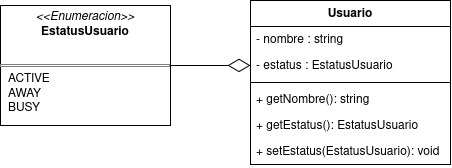
\includegraphics[scale=0.5]{UsuarioUML.png}\\
  \end{center}
\end{figure}

\subsection{Mensaje}
Tenemos también a los mensajes con los cuales el cliente se comunicara con el servidor y viceversa.\\

Como estos mensajes pueden tener diversos campos dependiendo su tipo, se puede hacer uso de el patron de diseño \textbf{Builder}, este patron ayudara a facilitar la construcción de los mensajes.\\

Los mensajes tienen campos como tipo, operacion, resultado, username, extra, estatus, users, text, roomname, usernames. Al ser más campos de los normales usar el patron de diseño Builder suele ser más claro.\\

Los campos como tipo, operacion, resultado, estatus, seran manejados como enumeraciones.\\

\begin{figure}[htb]
  \begin{center}
    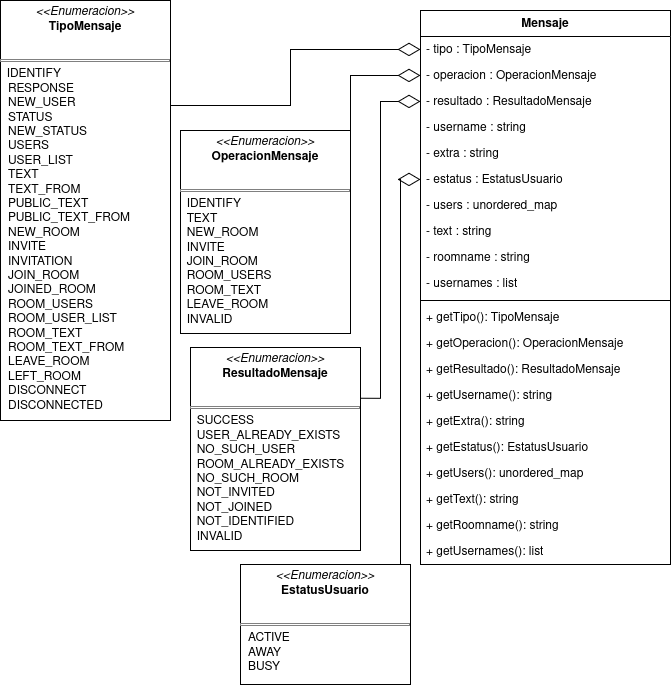
\includegraphics[scale=0.4]{MensajeUML.png}\\
  \end{center}
\end{figure}

\subsection{ValidaMensaje}
Podemos recibir un mensaje, sin embargo este puede no tener los elementos necesarios, estar incompleto o no ser valido, para eso tenemos \textit{ValidaMensaje}.\\

\subsection{GeneraMensaje}
Para poder facilitar la comunicación entre el cliente y el servidor, y que estos puedan saber que hacer facilmente, tenenmos la clase \textit{GeneraMensaje} que convertira los JSON recibidos a objetos de tipo Mensaje.\\

Y para facilitar el acceso usar una clase CampoMensaje.\\

\subsection{GeneraJSON}
Y ahora para que se puedan enviar los mensajes siguiendo el protocolo, convertirmos los objetos de tipo Mensaje a formato JSON para que el servidor lo pueda enviar al cliente y viceversa.\\

Al igual que GeneraMensaje también usara la clase CampoMensaje.\\

\subsection{Conexion}
Esta clase sera la que permita al cliente conectarse al servidor, y al servidor comunicarse con el cliente, sin que estos dos se comunique directamente, cuando el cliente envie algo, la conexión le avisara al servidor y cuando el servidor envie algo, entonces la conexión le avisara al cliente.\\

Con esto el servidor y el cliente decidiran que hacer, y que responder.\\

\subsection{Servidor}
Es uno de los elementos principales de este proyecto, este permitira la comunicación entre usuarios, si alguien, envia un mensaje el servidor se encargara de que a los demás usuarios les llegue ese mensaje o la respuesta a la acción hecha por el usuario.\\

Debe de procesar los mensajes que la conexión le informa que recibio, asi como tener el control de el chat, de los usuarios, de las salas, entre otros.\\

\subsection{Cliente}
El cliente sera el como el usuario se comunicara con el servidor y los demas usuarios, facilita todo el proceso de enviar los mensajes a unos simples metodos, esta clase también guardara la información del usuario, como su nombre y su estatus (mediante la clase Usuario).\\

Tendra también una conexión con la cual enviar mensajes y recibirlos.\\

\subsection{Controlador}
Esta clase sera mediante la cual el usuario haciendo uso de la interfaz podra realizar las solicitudes de las que se han estado hablado en este reporte.\\

Es una parte de el uso de el patron de diseño \textit{Modelo-Vista-Controlador}, donde el modelo seria el Cliente, la vista sera la interfaz.\\


\chapter{Implementación}
Con las clases ya propuestas, sus atributos y su comportamiento ya definido pasamos a la implementación de estas.\\

Necesitamos organizar nuestro espacio de trabajo y para eso haremos uso del sistema de construcción \textit{Meson}, que nos permitira poder compilar nuestro proyecto, generar los ejecutables y realizar pruebas unitarias haciento uso de \textit{GoogleTest}.

Podemos comenzar con la clase \textit{Usuario} siendo esta la más sencilla de implementar, esto permitio dar los primeros pasos para tener una implementación completa del proyecto.\\

Y como se desconocia el lenguaje \textit{C++} ayudo a dar también una introducción a este, y conforme se va avanzado se podra ir refactorizando para ajustar la clase a las necesidades exactas del proyecto.\\

Seguido de esto, se puede continuar con la clase \textit{Mensaje}, que seria la siguiente clase en dificultad, además que permitio aprender más sobre los patrones de diseño, como lo fue el caso de \textit{Builder} que después de su implementación facilito la implementación de la clases restantes para construir los mensajes necesarios.\\

Después de esto con los mensajes ya implementados podemos validarlos, y como se menciono, tenemos nuestra clase \textit{ValidaMensaje} que se encargara de checar si los mensajes recibidos son validos y poder realizar las operaciones correspondientes.\\

Esta clase hizo uso de metodos estaticos influyendo en la investigación de su funcionamiento en \textit{C++} y permitiendo hacer notar más las diferencias de este lenguaje con otro como Java o Python y sus diferentes formas de trabajar.\\

Debemos también poder generar mensajes en nuestro formato creador en nuestra clase mensaje, asi como también convertirlos a su forma JSON, para esto fue necesario tener una biblioteca JSON, y como \textit{C++} no tiene una por default, permitio manejar bibliotecas externas este caso usando \textit{Meson}, la biblioteca utilizada termino siendo \textit{JSON for Modern C++}.\\

Una vez esta parte lista, se pudo crear la conexión y haciendo más facil y rapida su implementación al tener todo lo anterior implementado y comenzando también con el uso de sockets.\\

Teniendo ya la conexión lista, se procedio a crear el servidor, implementando su comportamiento y que respondera antes los mensajes recibidos por los usuarios. Al no tener aun un cliente con el cual enviar mensajes, hicimos uso de \textit{telnet} para conectarnos a este permitiendonos avanzar con el proyecto y tener bien hecho el servidor.\\

Ya con esta parte lista procedimos a realizar el cliente para que el usuario pueda enviar mensajes, la implementación de los metodos resulto facil con todo lo que ya habiamos implementado anteriormente.\\

Finalmente, se procedio con la creación de la interfaz grafica, para esto hicimos uso de el framework \textit{Qt} y su lenguaje de marcado declarativo \textit{QML} que permitio implementar esta parte facilmente. A la vez que se iba implementando la interfaz y sus funciones fuimos creando el controlador, lo que nos permitio poco a poco ver un avance a todo lo que habiamos hecho y verlo en acción.\\

Una vez terminada la interfaz, realizamos pruebas usando otra computadora en la misma red, y con simplemente errores visuales, se tuvo exito al comunicarse entre los dos clientes.\\

\chapter{Conclusiones}
Al principio este proyecto se escuchaba dificil y dudaba de lo posible que seria poder realizar su implementación y más al no poder realizarlo en el unico lenguaje que maneja un poco bien (Java), sin embargo, el proyecto me ayudo a desarrollar aspectos de investigación, asi como mejorar la forma en la que implementaba mis clases y también haciendo pruebas unitarias un poco decentes.\\

Si pudiera mejorar algo de la implementación de mi proyecto seria principalmente la forma en la que implemente la comunicación entre el servidor y el cliente, además del diseño de la interfaz.\\

Al proyecto en general añadira un poco más de funciones como enviar imagenes aunque la dificultad de esto puede ser mayor para lo que busca el proyecto, pero si se podria dar más datos a los mensajes como la fecha y la hora, también se le podria dar más información al usuario además de solo su nombre y su estatus.\\

\chapter{Bibliografia}

Elisa Viso, Canek Peláez, Introducción a las Ciencias de la Computación con Java, Las prensas de Ciencias, 2012.\\

\url{https://tesiunamdocumentos.dgb.unam.mx/ptd2023/marzo/0836828/Index.html}\\

\url{https://www.geeksforgeeks.org/c/tcp-server-client-implementation-in-c/}\\

\end{document}
